\section{Experiments}
\label{sec:experiments}

% === Figures
\begin{table}[t]
  \begin{tabular}{l p{0.4\textwidth} p{0.4\textwidth} r r r}
    {\bf Dataset (Examples)} & {\bf Task and notes} & {\bf Features} \\ \hline
  {\bf NER (1000)}     & 
    We evaluate on a simplified version of CoNLL-2003 NER task\tablefootnote{\href{http://www.cnts.ua.ac.be/conll2003/ner/}{http://www.cnts.ua.ac.be/conll2003/ner/}}, a sequence labeling problem over English sentences. 
    We only consider the three entity tags corresponding to persons ($\textsc{per}$), locations ($\textsc{loc}$) or others ($\textsc{o}$)\tablefootnote{%
    The original also includes the tags $\textsc{org}$ and $\textsc{misc}$, however the distinctions between these tags are artificial, making it very difficult for non-expert crowd workers to provide accurate labels.}.
    &
    We used standard features~\cite{finkel2005incorporating}: the current word, current lemma, previous and next lemmas, lemmas in a window of size three to the left and right, word shape and word prefix and suffixes. \\
  {\bf Sentiment (1800)} & 
    We evaluate on a subset of the Stanford sentiment dataset\cite{maas2011learning} that consists of 2000 polar movie reviews; the goal is binary classification of documents into classes $\textsc{pos}$ and $\textsc{neg}$. 
    &
    We used two feature sets, the first (\textsc{bigrams}) containing only word unigrams and bigrams, and the second (\textsc{rnn}) that also contained sentence vector embeddings from~\cite{socher2013recursive}.
    \\
  {\bf Face (1784)} & 
  We evaluate on a celebrity face classification task\tablefootnote{\todo{}}. Each image must be labeled as one of the following four choices: Andersen Cooper, Daniel Craig, Scarlet Johansson and Miley Cyrus.
    &
    We used the last layer of a 11-layer AlexNet~\cite{krizhevsky2012imagenet} trained on ImageNet as input feature embeddings.
\end{tabular}
  \caption{Datasets used in this paper and number of examples we evaluate on.}
\label{tbl:dataset}
\end{table}

\begin{table}[t]
%% NER 
\begin{tabular}{l r r r r r | r r r r r}
  \multicolumn{6}{c|}{Named Entity Recognition} & 
      \multicolumn{3}{c}{Face Identification} \\
      \textbf{System} & \textbf{Latency} & \textbf{Qus./tok} & \textbf{P} & \textbf{R} & \textbf{F$_1$} 
          & \textbf{Latency} & \textbf{Qus./ex} & \textbf{Acc.} 
    \\ \hline
    1-vote & 664 ms & 1.0 & 66.38 & 89.58 & 76.15 
      & %1-vote & 
      1414 ms & 1.0 & 87.75 \\ %\hline
    3-vote & 1495 ms & 3.0 & 92.79 & 89.56 & 91.58 
        & %3-vote &
        1865 ms & 3.0 & 88.44 \\ %\hline
    5-vote & 3887 ms & 5.0 & 98.25 & 92.33 & 95.20 
        & 
        & -- & -- & -- \\
    Offline & n/a & n/a & 62.38 & 69.76 & 65.86 
        % Offline 
        & n/a & n/a & 87.43 \\    %\hline
    Entropic & 1523 ms & 0.65 & 91.74 & 90.90 & 91.33 
        % Entropic 
        & 1121 ms & 1.12 & \textbf{91.53} \\ %\hline
    \textbf{LENSE} & 3368 ms & \textbf{0.62} & \textbf{94.32} & \textbf{93.16} & \textbf{93.73} 
    %\textbf{LENSE} 
    & 961 ms & \textbf{1.06} & 88.45 \\   %\hline
\end{tabular}
\caption{Results on NER and Sentiment tasks comparing latencies, queries per token and performance metrics (Precision, Recall and \fone{} for NER and accuracy for Sentiment).}
\label{tbl:results}
\end{table}

\begin{table}[t]
    \begin{minipage}[t]{.49\textwidth }
        \begin{tabular}[b]{l  r  r  r  r}
    %\hline
    \textbf{System} & \textbf{Latency} & \textbf{Qu./ex} & \textbf{Acc.} \\ \hline
    1-vote & 6.6 s & 1.00 & 89.2 \\ %\hline
    3-vote & 10.9 s & 3.00 & 95.8 \\ %\hline
    5-vote & 13.5 s & 5.00 & 98.7 \\ %\hline
    \multicolumn{5}{c}{\textsc{bigrams}} \\ \hline
%Bigrams: \\
    Offline & n/a & n/a & TODO \\ %\hline
    \textbf{Threshold} & TODO s & TODO & TODO \\ %\hline
    LENSE & 18.1 s & 3.48 & 98.6 \\ %\hline
    \multicolumn{5}{c}{\textsc{rnn}} \\ \hline
    Offline & n/a & n/a & TODO \\ %\hline
    \textbf{Threshold} & 11.0 s & 2.85 & 96.0 \\ %\hline
    \textbf{LENSE} & 16.1 s & 3.19 & 98.6 \\% \hline
\end{tabular}

        \caption{Results on the Sentiment task comparing latency, queries per example and accuracy.}
        \label{tbl:sentiment-results}
        \vfill
    \end{minipage}%
    \begin{minipage}[t]{.49\textwidth}
  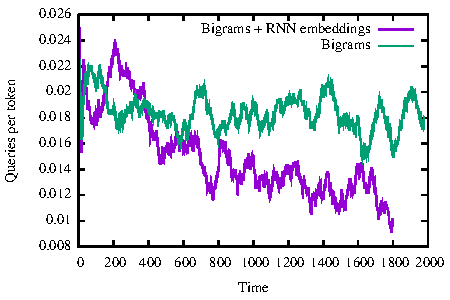
\includegraphics[width=\textwidth]{figures/sentiment_cost_per_token_vs_time/cost_per_token_vs_time.pdf}
  \captionof{figure}{Queries per example over time for the LENSE on Sentiment. With simple \textsc{bigram} features, the model does not have the capacity to predict at our desired accuracy and must query the crowd. With more complex \textsc{rnn} features, the model learns and queries the crowd less over time.}
        \label{fig:sentiment-tradeoff}
    \end{minipage}
\end{table}

% === Other stuff.

In this section, we empirically evaluate our approach on three tasks. 
While on-the-job setting we propose is targeted at scenarios where there is no data to begin with, we use existing labeled datasets (\tableref{dataset}) to empirically evaluate the performance of our system relative to baselines.

\paragraph{Baselines.}
We evaluated the following four methods on each dataset:
\begin{enumerate}
  \item {\bf Human n-query}: The majority vote of $n$ human crowd workers was used as a prediction.
  \item {\bf Offline baseline}:
    Uses a classifier that trains on the gold output for all examples seen so far and then returns the MLE as a prediction.
    This is the best possible offline system: it sees perfect information about all the data seen so far, but can not query the crowd while making a prediction.
  \item {\bf Entropic threshold}: Uses a heuristic on-the-job learning agent to make predictions. 
    The agent queries any labels that it estimates to have a marginal probability below a threshold $k = 0.88$. % \footnote{We found $k = 0.88$ to give the best results on our datasets.}
    Instead of computing the expected marginals over the responses to queries in flight, the agent simply reduces the uncertainty by a factor of $0.3$ and makes multiple requests until the threshold is crossed. Predictions are made using MLE on the model given responses.
    The agent does not reason about time and makes all its queries at the very beginning.
  \item {\bf LENSE:} Our full system as described in \sectionref{async}.
\end{enumerate}

To initialize parameters for the model-based methods, we used a burn-in period of 40 examples which were used to get labels on everything. We used those responses to train initial parameters for the prediction model $\theta$, response model $\beta$ and delay model $\Gamma$.
We do not update parameters for the delay and response models online.

\paragraph{Implementation and crowdsourcing setup.}
We implemented the retainer model of~\cite{bernstein2011crowds} on Amazon Mechanical Turk to create a ``pool'' of crowd workers that could respond to queries in real-time.
The workers were given a short tutorial on each task before joining the pool to minimize systematic errors caused by misunderstanding the task.
We paid Workers \$1.0 to join the retainer pool and an additional \$0.01 per query.
Worker response times were generally in the range of 3-6 seconds for NER, 10-15 seconds for Sentiment, and 2-4 seconds for Faces.

When running experiments, we found that the results varied based on the current worker quality. %, fluctuating on the NER task between 87 and 96 F1, depending on workers.
To control for variance in worker quality across our evaluations of the different methods, we collected 5 worker responses and their delays on each label ahead of time\footnote{If accepted, we will make our datasets of frozen human responses, delays, and anonymized worker tags publicly available}.
During simulation we sample the worker responses and delays without replacement from this frozen pool of worker responses. 
Neither LENSE nor the entropic threshold needed more than 3 queries on a single label.

% DETAILS
% Anecdotally, we also report a range of results on 5 complete runs of our system using {\em real live crowd workers}, recruited at test time, over the first 150 sentences of our dataset. The results exhibit high variance based on worker quality.
%
%\begin{center}
%\begin{tabular}{ | r | r | r | r | r | }
%    \hline
%    Time/token & Requests/token & Precision & Recall & F1 \\ \hline
%    1444 ms - 3426 ms & 0.54 - 0.66 & 92.9 - 96.91 & 82.50 - 94.01 & 87.4 - 95.43 \\ \hline
%\end{tabular}
%\end{center}
%
%Filtering workers while running, or inferring separate error models for each worker, would clearly deliver substantial gains in reliability over a system that assumes uniform quality. We leave this to future work.

\paragraph{Summary of results.}
\tableref{results} summarizes the performance of the methods on the three tasks.
On all three datasets, we found that on-the-job learning outperforms machine and human-only comparisons on both quality and cost. 
On NER, we achieve an \fone{} of $93.7\%$ at roughly 1/6th the cost of achieving the same result using the human-only approach. On Sentiment and Faces, we reduce costs for a comparable accuracy by a factor of 3-4.
For the latter two tasks, both on-the-job learning methods, entropic threshold baseline and LENSE, perform comparably.
The simple heuristic adopted by the entropic threshold baseline is sufficient to reason about expected marginals on both these tasks because they are single label prediction tasks which do not involve any interactions between labels.

\begin{figure}[t]
  \centering
  \begin{subfigure}[b]{0.49\textwidth}
  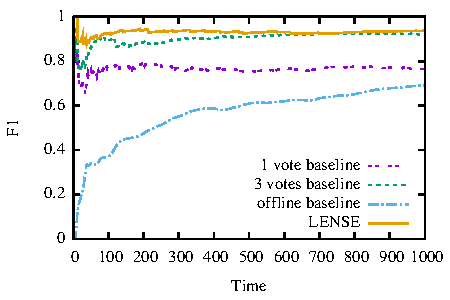
\includegraphics[width=\textwidth]{figures/ner_2_class/f1_plot/f1_vs_time.pdf}
\end{subfigure}
  \begin{subfigure}[b]{0.49\textwidth}
  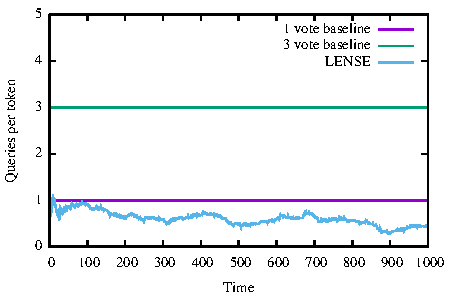
\includegraphics[width=\textwidth]{figures/ner_2_class/cost_plot/cost_vs_time.pdf}
  \end{subfigure}
  \caption{Comparing \fone{} and queries per token on the NER task. LENSE maintains high \fone{} scores by querying the crowd when it is unsure. As the model learns, it needs to query the crowd less.}
\label{fig:ner-f1}
\end{figure}

%\paragraph{Does the model respect accuracy preferences?} 
\figureref{ner-f1} tracks the performance and cost of LENSE over time on the NER task.
LENSE is not only able  to consistently outperform other baselines, but the cost of the system steadily reduces over time.
On the NER task, we find that LENSE is able to trade off time to produce more accurate results than the entropic threshold baseline with fewer queries by waiting for responses before making another query.

% == DEV F1
%We also plot \fone{} on a held-out set: while we receive noisy and sparse supervision LENSE is able to train a classifier that generalizes well over time. 
%Compared to the offline baseline, which sees perfect labels on all examples, LENSE observed labels on only \ac{KEENON: fix this number: 600} words. For a comparable number of tokens, the offline baseline has an \fone of \ac{KEENON: fix: 63\%}.

% === Compare with entropic threshold
%\paragraph{Why is the Entropic threshold system so much better on sentiment and faces?}
%LENSE exploits structure in the model when querying, and so outperforms the Entropic threshold in the presence of structure (see NER task results).
%However, when neither structure or time pressure is present, LENSE's only signal is the entropy of the prediction, and so the Entropic threshold is able to perform just as well, if not slightly better when the threshold is optimally set.

%We note that although our model is receiving supervisition signal at roughly 1/15 the rate of a fully observed online learning scenario\footnote{this calculation assumes ``fully observed'' is approximated by 3 human labels per example}, we track roughly parallel to the fully supervised line.

%\paragraph{In the limit, would LENSE still need crowd supervision?}
While on-the-job training allows us to deploy quickly and ensure good results, we would like to eventually operate without crowd supervision.
%In order to do so, we must ensure that our model has the capacity to keep learning from the crowd.
\figureref{sentiment-tradeoff}, we show the number of queries per example on Sentiment with two different features sets, \textsc{bigrams} and \textsc{rnn} (as described in \tableref{datasets}).
With simpler features (\textsc{bigrams}),
the model saturates early and we will continue to need to query to the crowd to achieve our accuracy target (as specified by the loss function).
On the other hand, using richer features (\textsc{rnn}) the model is able to learn from the crowd and the amount of supervision needed reduces over time.
%This suggests that given a sufficiently rich model, costs can be brought to zero in the limit.
Note that even when the model capacity is limited, LENSE is able to guarantee a consistent, high level of performance.

% -- CUT
%\paragraph{When does LENSE query?}
%During the initial stages of learning for the NER task, LENSE made multiple queries on all tokens.
%After a few examples, though, LENSE focused its queries on unseen entity tokens.
%Consider the following example taken from our run logs: \textit{``U.S.\ says still committed to Cuba migration pacts''}.
%%For example, after seeing \ac{600} examples, 
%The model has already seen {\it U.S.\/} and predicts that it is a \scloc{} with 97\% probability.
%On the other hand, having never seen the token {\it Cuba\/} before, the model starts with a belief that {\it Cuba\/} is 59\% \scper, 37\% \scloc{} and 3\% \scnone.
%It immediately fires off two queries about {\it Cuba\/} and waits 4 seconds for both responses to return \scloc{}.
%The model now believes that {\it Cuba\/} is \scloc{} with 95\% probability and returns its prediction.
%This demonstrates that using the model allows LENSE to focus supervision to where it is needed.


% \paragraph{Are we learning a good model?}
% We receive very noisy and sparse supervision.
% Despite this, to reduce the costs in the future, our system must learn to generalize well.
% We refer to \figureref{ner-dev-f1}.
% We note that although our model is receiving supervisition signal at roughly 1/15 the rate of a fully observed online learning scenario\footnote{this calculation assumes ``fully observed'' is approximated by 3 human labels per example}, we track roughly parallel to the fully supervised line.

% Held out figure for space concerns.
%\begin{figure}[t]
%  \begin{centering}
%  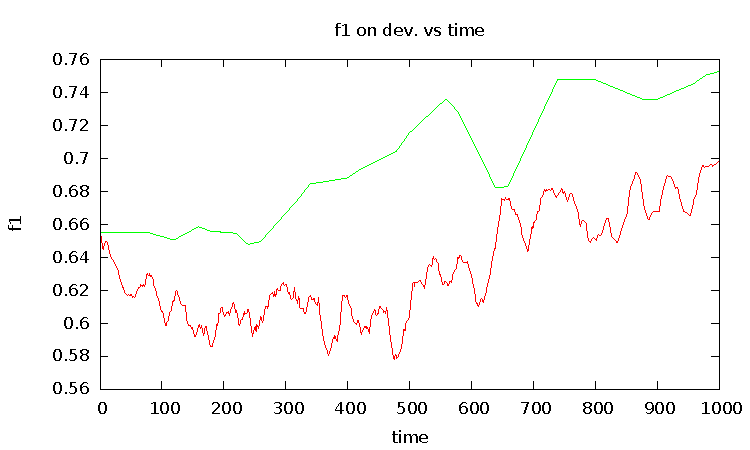
\includegraphics[width=1.0\textwidth]{figures/ner_2_class/machine_f1_plot/machine_f1_vs_time.pdf}
%  \end{centering}
%  \caption{A figure showing the relationship between the classifier we train, and one trained on gold labeled data. Evaluation is on a held out dev set. Note that our classifier learns more slowly because we are handing it a noisy approximation to train on, but the classifier narrows the gap as it gets more data.}
%\label{fig:ner-dev-f1}
%\end{figure}

